%%%%%%%%%%%%%%%%%%%%%%%%%%%%%%%%%%%%%%%%%
% Short Sectioned Assignment LaTeX Template Version 1.0 (5/5/12)
% This template has been downloaded from: http://www.LaTeXTemplates.com
% Original author:  Frits Wenneker (http://www.howtotex.com)
% License: CC BY-NC-SA 3.0 (http://creativecommons.org/licenses/by-nc-sa/3.0/)
%%%%%%%%%%%%%%%%%%%%%%%%%%%%%%%%%%%%%%%%%

%----------------------------------------------------------------------------------------
%	PACKAGES AND OTHER DOCUMENT CONFIGURATIONS
%----------------------------------------------------------------------------------------

\documentclass[paper=a4, fontsize=11pt]{scrartcl} % A4 paper and 11pt font size

% ---- Entrada y salida de texto -----

\usepackage[T1]{fontenc} % Use 8-bit encoding that has 256 glyphs
\usepackage[utf8]{inputenc}
%\usepackage{fourier} % Use the Adobe Utopia font for the document - comment this line to return to the LaTeX default

% ---- Idioma --------

\usepackage[spanish, es-tabla]{babel} % Selecciona el español para palabras introducidas automáticamente, p.ej. "septiembre" en la fecha y especifica que se use la palabra Tabla en vez de Cuadro

% ---- Otros paquetes ----

\usepackage{url} % ,href} %para incluir URLs e hipervínculos dentro del texto (aunque hay que instalar href)
\usepackage{hyperref}
\hypersetup{
	colorlinks=true,
	linkcolor=black,
	urlcolor=black,
	citecolor=black,
}
\usepackage{amsmath,amsfonts,amsthm} % Math packages
%\usepackage{graphics,graphicx, floatrow} %para incluir imágenes y notas en las imágenes
\usepackage{graphics,graphicx, float} %para incluir imágenes y colocarlas

% Para hacer tablas comlejas
%\usepackage{multirow}
%\usepackage{threeparttable}

%\usepackage{sectsty} % Allows customizing section commands
%\allsectionsfont{\centering \normalfont\scshape} % Make all sections centered, the default font and small caps

\usepackage{fancyhdr} % Custom headers and footers
\pagestyle{fancyplain} % Makes all pages in the document conform to the custom headers and footers
\fancyhead{} % No page header - if you want one, create it in the same way as the footers below
\fancyfoot[L]{} % Empty left footer
\fancyfoot[C]{} % Empty center footer
\fancyfoot[R]{\thepage} % Page numbering for right footer
\renewcommand{\headrulewidth}{0pt} % Remove header underlines
\renewcommand{\footrulewidth}{0pt} % Remove footer underlines
\setlength{\headheight}{13.6pt} % Customize the height of the header

\numberwithin{equation}{section} % Number equations within sections (i.e. 1.1, 1.2, 2.1, 2.2 instead of 1, 2, 3, 4)
\numberwithin{figure}{section} % Number figures within sections (i.e. 1.1, 1.2, 2.1, 2.2 instead of 1, 2, 3, 4)
\numberwithin{table}{section} % Number tables within sections (i.e. 1.1, 1.2, 2.1, 2.2 instead of 1, 2, 3, 4)

\setlength\parindent{0pt} % Removes all indentation from paragraphs - comment this line for an assignment with lots of text

\newcommand{\horrule}[1]{\rule{\linewidth}{#1}} % Create horizontal rule command with 1 argument of height
\usepackage{booktabs}

\usepackage{listings}
\lstdefinelanguage
[x64]{Assembler}     % add a "x64" dialect of Assembler
[x86masm]{Assembler} % based on the "x86masm" dialect
{morekeywords={CDQE,CQO,CMPSQ,CMPXCHG16B,JRCXZ,LODSQ,MOVSXD, %
		POPFQ,PUSHFQ,SCASQ,STOSQ,IRETQ,RDTSCP,SWAPGS, %
		rax,rdx,rcx,rbx,rsi,rdi,rsp,rbp, %
		r8,r8d,r8w,r8b,r9,r9d,r9w,r9b, %
		r10,r10d,r10w,r10b,r11,r11d,r11w,r11b, %
		r12,r12d,r12w,r12b,r13,r13d,r13w,r13b, %
		r14,r14d,r14w,r14b,r15,r15d,r15w,r15b}} % etc.
\usepackage{color}
\usepackage{xcolor}
\lstdefinestyle{customc}{
	belowcaptionskip=1\baselineskip,
	breaklines=true,
	frame=L,
	xleftmargin=\parindent,
	language=C,
	showstringspaces=false,
	basicstyle=\footnotesize\ttfamily,
	keywordstyle=\bfseries\color{green!40!black},
	commentstyle=\itshape\color{purple!40!black},
	identifierstyle=\color{blue},
	stringstyle=\color{orange},
}

\lstset{escapechar=@,style=customc}
\usepackage{url}

\title{	
	\normalfont \normalsize
	\begin{figure}[htb]
		\centering
		
\includegraphics[width=0.3\textwidth]{./imagenes/1}
	\end{figure}
	\textsc{\textbf{Estructura de Computadores} \\ Grado en Ingeniería Informática \\ 
	Curso 2018-2019} \\ [25pt] % Your university, school and/or department name(s)
	\begin{figure}[htb]
		\centering
		
\includegraphics[width=0.15\textwidth]{./imagenes/2}
	\end{figure}
	\horrule{0.5pt} \\[0.4cm] % Thin top horizontal rule
	\huge Memoria Práctica 3. \\
	\huge Programaci\'on mixta C-asm x86-64 Linux.
	\\ % The assignment title
	\horrule{2pt} \\[0.5cm] % Thick bottom horizontal rule
}
\author{Félix Ramírez García  \\
\href{mailto:felixramirezgarcia@correo.ugr.es}{felixramirezgarcia@correo.ugr.es}} % Nombre y apellidos
\date{\normalsize\today} % Incluye la fecha actual

%----------------------------------------------------------------------------------------
% DOCUMENTO
%----------------------------------------------------------------------------------------

\begin{document}
	
	\maketitle % Muestra el Título
	
	\newpage %inserta un salto de página
	
	\tableofcontents % para generar el índice de contenidos
	
	\listoffigures % para generar índice de imágenes.
	
	\listoftables % para generar índice de tablas.
	
	\newpage
	
	%-----------------------------------------------------------------------
	%							Diario de trabajo
	%----------------------------------------------------------------------	
	\section[Diario de trabajo]{Diario de trabajo.}
		
	\begin{table}[htbp]
		\begin{center}
			\begin{tabular}{|l|l|}
				\hline
				Fecha & Tarea desarrollada \\
				\hline \hline
				29-10-2018 & Repaso de la parte A del guion de la práctica \\ \hline
				30-10-2018 & Lectura de la parte B del guion de la práctica \\ \hline
				31-11-2018 & Terminados los popcounts 1,2,3 \\ \hline
				1-11-2018 & Intento de popcount4 y terminados popcounts 5,6,7,8 \\ \hline
				2-11-2018 & Popcount 9 y 10 , test , hoja de calculo y gráfica\\ \hline
			\end{tabular}
			\caption{Diario de trabajo de la práctica.}
			\label{tabla:sencilla}
		\end{center}
	\end{table}
	
	%-----------------------------------------------------------------------
	%							codigo de los programas
	%-----------------------------------------------------------------------
	\section[Código de los ejercicios]{Código de los ejercicios}
	
	%-----------------------------------------------------------------------
	%-----------------------------------------------------------------------
	
	\subsection{Calcular la suma de bits de una lista de enteros sin signo}
	
	\lstset{language=C}
	\begin{lstlisting}[frame=single]
#include <stdio.h>		
#include <stdlib.h>		
#include <sys/time.h>

#define WSIZE (8*sizeof(int))

#ifndef TEST 
#define TEST 5 
#endif 

//------------------------------------------
#if TEST==1 
#define SIZE 4
unsigned lista[SIZE]={0x80000000, 0x00400000, 0x00000200, 0x00000001};   
#define RESULT 4 
//------------------------------------------
#elif TEST==2 
#define SIZE 8
unsigned lista[SIZE]={0x7fffffff, 0xffefffff, 0xfffff7ff, 0xfffffffe, 0x01000024, 0x00356700, 0x8900ac00, 0x00bd00ef};   
#define RESULT 156
//------------------------------------------
#elif TEST==3
#define SIZE 8
unsigned lista[SIZE]={0x0	   , 0x10204080, 0x3590ac06, 0x70b0d0e0, 0xffffffff ,0x12345678, 0x9abcdef0, 0xcafebeef};   
#define RESULT 116
//------------------------------------------
#elif TEST==4 || TEST==0 
#define NBITS 20
#define SIZE (1<<NBITS)
unsigned lista[SIZE];
#define RESULT (NBITS*(1<<NBITS-1))
//------------------------------------------
#else 
#error "Definir TEST entre 0..4" 
#endif

// Primera version del popcount: recorremos array y bits con for
unsigned popcount1(int* array, int len){

int i;
int j;
unsigned result = 0;
unsigned x;
// Para todos los numeros del vector
for(i = 0; i < len; i++) {	      		    
x = array[i];					      	// Extraemos un numero

for(j = 0; j < WSIZE; j++){    	    	// Recorremos todos los bits del numero.
unsigned mascara = 1 << j; 			// Extraemos los bits con una mascara 0x1
result += (x & mascara) != 0; 		// Vamos acumulando el resultado
}
}
return result;
}

// Segunda version del popcount: recorremos array con for y bits con while
unsigned popcount2(int* array, int len){

int i;
unsigned x;
unsigned result = 0;

for(i = 0; i < len; i++) {    // Recorremos el vector
x = array[i];			  // Extraemos un numero

while (x) {			  // Recorremos todos los bits de dicho numero
result += x&0x1; 	  // Extraemos los bits con una mascara 0x1 y
// los acumulamos en el contador "resultado"
x >>= 1;			  // Realizamos el desplazamiento de bits a la dcha
}
}
return result;
}

// Tercera version del popcount: recorremos el array con for y bits con asm (orden adc)
unsigned popcount3(unsigned *array, int len){

int i;
unsigned result = 0;
unsigned x;

for(i = 0; i < len; i++){
x = array[i];
asm( 				   "\n"
"ini3:				  \n\t"	   	// Seguiremos mientras num != 0
"shr  %[x]			  \n\t"	   	// LSB en CF
"adc  $0, 	%[result] \n\t"	   	// Acumulamos el acarreo
"test %[x], %[x]	  \n\t"	   	// Comprobamos si num != 0
"jnz  ini3			  \n\t"	   	// Hacemos el salto si quedan bits a 1
: [result]"+r" (result)			// E/S: aniadir lo acumulado por el momento
: [x] "r" (x)  			   		// entrada: valor elemento
);
}
return result;
}


// Quinta version del popcount: recorremos con for anidado y la suma en arbol
unsigned popcount5(unsigned *array, int len){

int i;
int j;
unsigned val = 0;
unsigned result = 0;
unsigned x;

for(i = 0; i < len; i++){     // Recorremos el vector
x = array[i];			  // Escogemos un numero del vector

for(j = 0; j < 8; j++){	  // Recorremos los bytes
val += x & 0x01010101;	  // Acumulamos los bits de cada byte recorrido
x >> 1;					  // Realizamos el desplazamiento a la dcha
}

val += (val >> 16);		  // Volvemos a acumular en "valor" mientras desplazamos
val += (val >> 8);		  // Volvemos a acumular en "valor" mientras desplazamos

result += (val & 0xFF);   // Acumulamos todo en "resultado"
val = 0; 			 	  // Volvemos a poner a cero la variable valor
// y volvemos a empezar el bucle
}
return result;
}

// Sexta version del popcount: version naive de Wikipedia aplicada a array
int popcount64a(unsigned x) {     
x = (x & 0x5555555555555555 ) + ((x >>  1) & 0x5555555555555555 ); //put count of each  2 bits into those  2 bits      
x = (x & 0x3333333333333333 ) + ((x >>  2) & 0x3333333333333333 ); //put count of each  4 bits into those  4 bits     
x = (x & 0x0f0f0f0f0f0f0f0f ) + ((x >>  4) & 0x0f0f0f0f0f0f0f0f ); //put count of each  8 bits into those  8 bits      
x = (x & 0x00ff00ff00ff00ff ) + ((x >>  8) & 0x00ff00ff00ff00ff ); //put count of each 16 bits into those 16 bits      
x = (x & 0x0000ffff0000ffff ) + ((x >> 16) & 0x0000ffff0000ffff ); //put count of each 32 bits into those 32 bits      
x = (x & 0x00000000ffffffff ) + ((x >> 32) & 0x00000000ffffffff ); //put count of each 64 bits into those 64 bits      
return x; 
} 
unsigned popcount6(unsigned *array, int len){

int i;
unsigned result = 0;
unsigned x;

for(i = 0; i < len; i++){     // Recorremos el vector
x = array[i];
result += popcount64a(x);
}
return result;
}

// Septima version del popcount: version naive de Wikipedia aplicada a array con desenrollado de bucle
unsigned popcount7(unsigned *array, int len){

int i;
unsigned result = 0;
unsigned x1, x2, x3, x4;

for(i = 0; i < len; i+=4){     // Recorremos el vector
x1 = array[i];
x2 = array[i+1];
x3 = array[i+2];
x4 = array[i+3];
result += popcount64a(x1) + popcount64a(x2) + popcount64a(x3) + popcount64a(x4);
}
return result;
}

// Octava version del popcount: SSE3
unsigned popcount8 (unsigned *array, int len){

int i;
unsigned val;
unsigned result = 0;
int SSE_mascara[] = {0x0f0f0f0f, 0x0f0f0f0f, 0x0f0f0f0f, 0x0f0f0f0f};
int SSE_LUTb[] = {0x02010100, 0x03020201, 0x03020201, 0x04030302};

if (len & 0x3)
printf("leyendo 128b pero len no multiplo de 4?\n");

for (i = 0; i < len; i += 4){
asm(
"movdqu 	%[x], 	%%xmm0 	\n\t"
"movdqa		%%xmm0, %%xmm1	\n\t"	// Creamos dos copias de x
"movdqu 	%[m], 	%%xmm6	\n\t"	// Creamos la mascara
"psrlw		$4, 	%%xmm1 	\n\t"
"pand 		%%xmm6, %%xmm0	\n\t"	// xmm0 - nibbles inferiores
"pand		%%xmm6, %%xmm1	\n\t"	// xmm1 - nibbles superiores

"movdqu		%[l],	%%xmm2	\n\t"	// ...como pshufb sobrescribe LUT
"movdqa		%%xmm2, %%xmm3	\n\t"	// ...queremos 2 copias
"pshufb		%%xmm0,	%%xmm2	\n\t"	// xmm2 = vector popcount inferiores
"pshufb		%%xmm1,	%%xmm3	\n\t"	// xmm3 = vector popcount superiores

"paddb		%%xmm2, %%xmm3	\n\t"	// xmm2 += xmm3 - vector popcount bytes
"pxor		%%xmm0, %%xmm0	\n\t"	// xmm0 = 0,0,0,0
"psadbw		%%xmm0, %%xmm3	\n\t"	// xmm3 = [pcnt bytes0..7|pcnt bytes8..15]
"movhlps	%%xmm3,	%%xmm0	\n\t"	// xmm0 = [	0 		  |pcnt bytes0..7]
"paddd		%%xmm3,	%%xmm0	\n\t"	// xmm0 = [	no usado  |pcnt bytes0..15]
"movd 		%%xmm0, %[val]\n\t"
: [val]"=r" (val)
: [x]  "m"	(array[i]),
[m]  "m"	(SSE_mascara[0]),
[l]  "m"	(SSE_LUTb[0])
);
result += val;
}
return result;
}

// Novena version del popcount: implementando la instruccion SSE4
unsigned popcount9 (unsigned *array, int len){
unsigned x;
int i;
unsigned val;
unsigned result = 0;

for (i = 0; i < len; i++){
x = array[i];
asm(
"popcnt     %[x],   %[val] 	\n\t"
: [val]"=r" (val)
: [x]  "r"	(x)
);

result += val;
}
return result;
}

//Decima version del popcount, implementando la instruccion SSE4 con desenrollado
unsigned popcount10 (unsigned *array, int len){
unsigned x1,x2,x3,x4;
int i;
unsigned val1,val2,val3,val4;
unsigned result = 0;

for (i = 0; i < len; i+=4){
x1 = array[i];
x2 = array[i+1];
x3 = array[i+2];
x4 = array[i+3];
asm(
"popcnt     %[x1],   %[val1] 	\n\t"
"popcnt     %[x2],   %[val2] 	\n\t"
"popcnt     %[x3],   %[val3] 	\n\t"
"popcnt     %[x4],   %[val4] 	\n\t"
: [val1]"=r" (val1),
[val2]"=r" (val2),
[val3]"=r" (val3),
[val4]"=r" (val4)
: [x1]  "r"	(x1),
[x2]  "r"	(x2),
[x3]  "r"	(x3),
[x4]  "r"	(x4)
);

result += val1 + val2 +val3 +val4;
}
return result;
}

// Funcion cronometro para calcular los tiempos
void crono(unsigned (*func)(), char* msg){

struct timeval tv1,tv2;		// gettimeofday() secs-usecs
long tv_usecs;			    // y sus cuentas

gettimeofday(&tv1, NULL);
unsigned resultado = func(lista, SIZE);
gettimeofday(&tv2, NULL);

tv_usecs = (tv2.tv_sec - tv1.tv_sec )*1E6 + (tv2.tv_usec - tv1.tv_usec);

#if TEST==0
printf(    "%ld" "\n",      tv_usecs); 
#else     
printf("resultado = %d\t", resultado);     
printf("%s:%9ld us\n", msg, tv_usecs); 
#endif 
}

//Funcion main que cronometra los tiempos de todas las funciones
int main(){

#if TEST==0 || TEST==4     
size_t i;     // inicializar array     
for (i=0; i<SIZE; i++)   
lista[i]=i; 
#endif 

crono(popcount1, "popcount1, lenguaje C - for");
crono(popcount2, "popcount2, lenguaje C - while");
crono(popcount3, "popcount3, leng.ASM-body while 4i");
crono(popcount5, "popcount5, CS:APP2e 3.49-group 8b");
crono(popcount6, "popcount6, Wikipedia- naive - 32b");
crono(popcount7, "popcount7, Wikipedia- naive - 128b");
crono(popcount8, "popcount8, asm SSE3 - pshufb 128b");
crono(popcount9, "popcount9, asm SSE4 - pshufb 32b");
crono(popcount10, "popcount10, asm SSE4 - pshufb 128b");


#if TEST != 0     
printf("calculado = %d\n", RESULT); 
#endif 

exit(0);
}
	\end{lstlisting}
	
	%-----------------------------------------------------------------------
	%							Pruebas de ejecución
	%-----------------------------------------------------------------------
	\section[Pruebas de ejecución]{Pruebas de ejecución}

	\lstset{language=C}
	\begin{lstlisting}[frame=single]  
__OPTIM0__================================================ 
__TEST01__------------------------------------------------
resultado = 4	popcount1, lenguaje C - for:        1 us
resultado = 4	popcount2, lenguaje C - while:        1 us
resultado = 4	popcount3, leng.ASM-body while 4i:        1 us
resultado = 8	popcount5, CS:APP2e 3.49-group 8b:        1 us
resultado = 8	popcount6, Wikipedia- naive - 32b:        1 us
resultado = 8	popcount7, Wikipedia- naive - 128b:        0 us 
resultado = 4	popcount8, asm SSE3 - pshufb 128b:        0 us
resultado = 4	popcount9, asm SSE4 - pshufb 32b:        0 us
resultado = 4	popcount10, asm SSE4 - pshufb 128b:        0 us
calculado = 4
__TEST02__------------------------------------------------
resultado = 156	popcount1, lenguaje C - for:        1 us
resultado = 156	popcount2, lenguaje C - while:        2 us
resultado = 156	popcount3, leng.ASM-body while 4i:        0 us
resultado = 168	popcount5, CS:APP2e 3.49-group 8b:        0 us
resultado = 312	popcount6, Wikipedia- naive - 32b:        0 us
resultado = 312	popcount7, Wikipedia- naive - 128b:        0 us
resultado = 156	popcount8, asm SSE3 - pshufb 128b:        0 us
resultado = 156	popcount9, asm SSE4 - pshufb 32b:        0 us
resultado = 88	popcount10, asm SSE4 - pshufb 128b:        0 us
calculado = 156
__TEST03__------------------------------------------------
resultado = 116	popcount1, lenguaje C - for:        2 us
resultado = 116	popcount2, lenguaje C - while:        0 us
resultado = 116	popcount3, leng.ASM-body while 4i:        1 us
resultado = 48	popcount5, CS:APP2e 3.49-group 8b:        0 us
resultado = 232	popcount6, Wikipedia- naive - 32b:        0 us
resultado = 232	popcount7, Wikipedia- naive - 128b:        0 us
resultado = 116	popcount8, asm SSE3 - pshufb 128b:        0 us
resultado = 116	popcount9, asm SSE4 - pshufb 32b:        0 us
resultado = 54	popcount10, asm SSE4 - pshufb 128b:        0 us
calculado = 116
__TEST04__------------------------------------------------
resultado = 10485760	popcount1, lenguaje C - for:    74055 us
resultado = 10485760	popcount2, lenguaje C - while:    35838 us
resultado = 10485760	popcount3, leng.ASM-body while 4i:    11468 us
resultado = 12582912	popcount5, CS:APP2e 3.49-group 8b:    14431 us
resultado = 20971520	popcount6, Wikipedia- naive - 32b:    10565 us
resultado = 20971520	popcount7, Wikipedia- naive - 128b:     8000 us
resultado = 10485760	popcount8, asm SSE3 - pshufb 128b:      822 us
resultado = 10485760	popcount9, asm SSE4 - pshufb 32b:     3922 us
resultado = 6121176	popcount10, asm SSE4 - pshufb 128b:     1512 us
calculado = 10485760
__OPTIMg__================================================
__TEST01__------------------------------------------------
resultado = 4	popcount1, lenguaje C - for:        1 us
resultado = 4	popcount2, lenguaje C - while:        0 us
resultado = 4	popcount3, leng.ASM-body while 4i:        0 us
resultado = 8	popcount5, CS:APP2e 3.49-group 8b:        0 us
resultado = 4	popcount6, Wikipedia- naive - 32b:        0 us
resultado = 4	popcount7, Wikipedia- naive - 128b:        1 us
resultado = 4	popcount8, asm SSE3 - pshufb 128b:        1 us
resultado = 4	popcount9, asm SSE4 - pshufb 32b:        0 us
resultado = 4	popcount10, asm SSE4 - pshufb 128b:        0 us
calculado = 4
__TEST02__------------------------------------------------
resultado = 156	popcount1, lenguaje C - for:        1 us
resultado = 156	popcount2, lenguaje C - while:        1 us
resultado = 156	popcount3, leng.ASM-body while 4i:        1 us
resultado = 168	popcount5, CS:APP2e 3.49-group 8b:        1 us
resultado = 156	popcount6, Wikipedia- naive - 32b:        0 us
resultado = 156	popcount7, Wikipedia- naive - 128b:        0 us
resultado = 156	popcount8, asm SSE3 - pshufb 128b:        0 us
resultado = 156	popcount9, asm SSE4 - pshufb 32b:        0 us
resultado = 156	popcount10, asm SSE4 - pshufb 128b:        1 us
calculado = 156
__TEST03__------------------------------------------------
resultado = 116	popcount1, lenguaje C - for:        0 us
resultado = 116	popcount2, lenguaje C - while:        1 us
resultado = 116	popcount3, leng.ASM-body while 4i:        0 us
resultado = 48	popcount5, CS:APP2e 3.49-group 8b:        0 us
resultado = 116	popcount6, Wikipedia- naive - 32b:        0 us
resultado = 116	popcount7, Wikipedia- naive - 128b:        0 us
resultado = 116	popcount8, asm SSE3 - pshufb 128b:        0 us
resultado = 116	popcount9, asm SSE4 - pshufb 32b:        0 us
resultado = 116	popcount10, asm SSE4 - pshufb 128b:        0 us
calculado = 116
__TEST04__------------------------------------------------
resultado = 10485760	popcount1, lenguaje C - for:    28145 us
resultado = 10485760	popcount2, lenguaje C - while:    11357 us
resultado = 10485760	popcount3, leng.ASM-body while 4i:     9740 us
resultado = 12582912	popcount5, CS:APP2e 3.49-group 8b:     4203 us
resultado = 10485760	popcount6, Wikipedia- naive - 32b:     2661 us
resultado = 10485760	popcount7, Wikipedia- naive - 128b:     2302 us
resultado = 10485760	popcount8, asm SSE3 - pshufb 128b:      398 us
resultado = 10485760	popcount9, asm SSE4 - pshufb 32b:      585 us
resultado = 10485760	popcount10, asm SSE4 - pshufb 128b:      347 us
calculado = 10485760
__OPTIM1__================================================
__TEST01__------------------------------------------------
resultado = 4	popcount1, lenguaje C - for:        1 us
resultado = 4	popcount2, lenguaje C - while:        1 us
resultado = 4	popcount3, leng.ASM-body while 4i:        1 us
resultado = 8	popcount5, CS:APP2e 3.49-group 8b:        0 us
resultado = 4	popcount6, Wikipedia- naive - 32b:        1 us
resultado = 4	popcount7, Wikipedia- naive - 128b:        1 us
resultado = 4	popcount8, asm SSE3 - pshufb 128b:        0 us
resultado = 4	popcount9, asm SSE4 - pshufb 32b:        0 us
resultado = 4	popcount10, asm SSE4 - pshufb 128b:        0 us
calculado = 4
__TEST02__------------------------------------------------
resultado = 156	popcount1, lenguaje C - for:        1 us
resultado = 156	popcount2, lenguaje C - while:        1 us
resultado = 156	popcount3, leng.ASM-body while 4i:        0 us
resultado = 168	popcount5, CS:APP2e 3.49-group 8b:        0 us
resultado = 156	popcount6, Wikipedia- naive - 32b:        1 us
resultado = 156	popcount7, Wikipedia- naive - 128b:        1 us
resultado = 156	popcount8, asm SSE3 - pshufb 128b:        1 us
resultado = 156	popcount9, asm SSE4 - pshufb 32b:        0 us
resultado = 156	popcount10, asm SSE4 - pshufb 128b:        0 us
calculado = 156
__TEST03__------------------------------------------------
resultado = 116	popcount1, lenguaje C - for:        1 us
resultado = 116	popcount2, lenguaje C - while:        0 us
resultado = 116	popcount3, leng.ASM-body while 4i:        1 us
resultado = 48	popcount5, CS:APP2e 3.49-group 8b:        1 us
resultado = 116	popcount6, Wikipedia- naive - 32b:        1 us
resultado = 116	popcount7, Wikipedia- naive - 128b:        1 us
resultado = 116	popcount8, asm SSE3 - pshufb 128b:        1 us
resultado = 116	popcount9, asm SSE4 - pshufb 32b:        1 us
resultado = 116	popcount10, asm SSE4 - pshufb 128b:        1 us
calculado = 116
__TEST04__------------------------------------------------
resultado = 10485760	popcount1, lenguaje C - for:    27435 us
resultado = 10485760	popcount2, lenguaje C - while:     9809 us
resultado = 10485760	popcount3, leng.ASM-body while 4i:    11179 us
resultado = 12582912	popcount5, CS:APP2e 3.49-group 8b:     2965 us
resultado = 10485760	popcount6, Wikipedia- naive - 32b:     2424 us
resultado = 10485760	popcount7, Wikipedia- naive - 128b:     2400 us
resultado = 10485760	popcount8, asm SSE3 - pshufb 128b:      391 us
resultado = 10485760	popcount9, asm SSE4 - pshufb 32b:      422 us
resultado = 10485760	popcount10, asm SSE4 - pshufb 128b:      297 us
calculado = 10485760
__OPTIM2__================================================
__TEST01__------------------------------------------------
resultado = 4	popcount1, lenguaje C - for:        0 us
resultado = 4	popcount2, lenguaje C - while:        0 us
resultado = 4	popcount3, leng.ASM-body while 4i:        1 us
resultado = 8	popcount5, CS:APP2e 3.49-group 8b:        1 us
resultado = 4	popcount6, Wikipedia- naive - 32b:        1 us
resultado = 4	popcount7, Wikipedia- naive - 128b:        1 us
resultado = 4	popcount8, asm SSE3 - pshufb 128b:        1 us
resultado = 4	popcount9, asm SSE4 - pshufb 32b:        0 us
resultado = 4	popcount10, asm SSE4 - pshufb 128b:        0 us
calculado = 4
__TEST02__------------------------------------------------
resultado = 156	popcount1, lenguaje C - for:        1 us
resultado = 156	popcount2, lenguaje C - while:        1 us
resultado = 156	popcount3, leng.ASM-body while 4i:        0 us
resultado = 168	popcount5, CS:APP2e 3.49-group 8b:        0 us
resultado = 156	popcount6, Wikipedia- naive - 32b:        0 us
resultado = 156	popcount7, Wikipedia- naive - 128b:        0 us
resultado = 156	popcount8, asm SSE3 - pshufb 128b:        0 us
resultado = 156	popcount9, asm SSE4 - pshufb 32b:        0 us
resultado = 156	popcount10, asm SSE4 - pshufb 128b:        0 us
calculado = 156
__TEST03__------------------------------------------------
resultado = 116	popcount1, lenguaje C - for:        1 us
resultado = 116	popcount2, lenguaje C - while:        1 us
resultado = 116	popcount3, leng.ASM-body while 4i:        1 us
resultado = 48	popcount5, CS:APP2e 3.49-group 8b:        0 us
resultado = 116	popcount6, Wikipedia- naive - 32b:        1 us
resultado = 116	popcount7, Wikipedia- naive - 128b:        0 us
resultado = 116	popcount8, asm SSE3 - pshufb 128b:        0 us
resultado = 116	popcount9, asm SSE4 - pshufb 32b:        1 us
resultado = 116	popcount10, asm SSE4 - pshufb 128b:        1 us
calculado = 116
__TEST04__------------------------------------------------
resultado = 10485760	popcount1, lenguaje C - for:    23239 us
resultado = 10485760	popcount2, lenguaje C - while:     8800 us
resultado = 10485760	popcount3, leng.ASM-body while 4i:     9202 us
resultado = 12582912	popcount5, CS:APP2e 3.49-group 8b:      971 us
resultado = 10485760	popcount6, Wikipedia- naive - 32b:     2445 us
resultado = 10485760	popcount7, Wikipedia- naive - 128b:     2587 us
resultado = 10485760	popcount8, asm SSE3 - pshufb 128b:      455 us
resultado = 10485760	popcount9, asm SSE4 - pshufb 32b:      467 us
resultado = 10485760	popcount10, asm SSE4 - pshufb 128b:      311 us
calculado = 10485760
__OPTIM0__================================================

2018-11-02 18:17                                                          Page 1

0      1      2	     3	    4	   5	  6	 7	8      9      10
73915  73874  75326  73500  74411  73421  74241	 73449	73946  73965  74185
35619  36796  37419  36574  35661  38637  35551	 36763	35769  36459  36099
11409  11255  11166  11168  11217  11154  11585	 11166	11183  11030  11260
15129  14499  14856  14504  14587  14547  14684	 14626	14841  14627  14595
10521  10853  10669  10597  10366  10456  10708	 10447	10365  10496  10723
8015   7885   8256   8000   8064   8102	  8068	 8014	8166   7887   8206
806    860    827    858    906	   814	  811	 818	870    811    817
2475   2502   2602   2488   2746   2569	  2453	 2454	2586   2490   2473
1465   1454   1457   1480   1592   1473	  1474	 1544	1459   1461   1493

__OPTIMg__================================================

2018-11-02 18:17                                                          Page 1

0      1      2	     3	    4	   5	  6	 7	8      9      10
26671  26003  27956  27614  27654  28342  28479	 26032	25134  25896  26168
11970  11171  11255  15654  11451  11314  11120	 11226	11220  11470  11623
9268   9231   9707   10037  9382   9469	  9320	 9653	9365   9368   9431
4125   4194   4124   4220   4272   4470	  4464	 4215	4345   4234   4295
2555   2560   2693   2576   2666   2685	  2592	 2590	2566   2698   2560
2313   2302   2302   2385   2319   2297	  2387	 2420	2301   2321   2306
382    387    354    420    377	   357	  382	 478	352    371    374
656    581    594    632    580	   590	  621	 614	757    581    604
322    300    302    330    308	   304	  290	 358	401    303    349

__OPTIM1__================================================

2018-11-02 18:17                                                          Page 1

0      1      2	     3	    4	   5	  6	 7	8      9      10
28281  29709  28140  27065  27456  27622  27016	 27014	26846  27636  27386
10479  10521  10641  10374  9393   10535  10283	 10377	10810  9940   9975
10901  10892  10883  11046  10828  11061  10838	 11208	11024  10932  11151
2871   2819   2798   2816   2796   2891	  2799	 3048	2793   2802   2799
2502   2436   2578   2481   2413   2454	  2414	 2437	2424   2417   2541
2435   2391   2390   2529   2400   2391	  2389	 2391	2397   2399   2388
404    366    356    403    367	   411	  361	 381	358    356    361
454    420    429    484    428	   431	  426	 418	416    428    415
313    323    309    328    302	   318	  333	 296	314    294    310

__OPTIM2__================================================

2018-11-02 18:17                                                          Page 1

0      1      2	     3	    4	   5	  6	 7	8      9      10
28399  29238  29821  27792  29290  29676  31071	 29646	28900  27675  29017
7408   7857   8221   7219   7297   7265	  7219	 7243	7239   8299   7274
9263   9181   9394   9175   9243   9167	  9262	 9230	9110   9405   9219
1023   993    955    1031   970	   994	  1013	 1078	985    1014   991
2390   2354   2374   2407   2348   2347	  2343	 2352	2390   2359   2390
2329   2243   2335   2290   2279   2202	  2361	 2271	2210   2208   2276
363    383    419    397    363	   353	  381	 392	368    355    373
406    407    434    435    412	   413	  431	 422	407    418    415
294    281    326    360    304	   296	  281	 296	293    295    296
	\end{lstlisting}

	%-----------------------------------------------------------------------
	%							Script de ejecución
	%-----------------------------------------------------------------------
	\section[Script de ejecución]{Script de ejecución}

	\lstset{language=bash}
	\begin{lstlisting}[frame=single] 
for i in 0 g 1 2; do 
	printf "__OPTIM%1c__%48s\n" $i "" | tr " " "="
	for j in $(seq 1 4); do 
		printf "__TEST%02d__%48s\n" $j "" | tr " " "-"       
		rm  popcount       
		gcc popcount.c -w -o popcount -O$i -D TEST=$j -g         
		./popcount     
	done   
done  

for i in 0 g 1 2; do        
	printf "__OPTIM%1c__%48s\n" $i "" | tr " " "="       
	rm  popcount       
	gcc popcount.c -w -o popcount -O$i -D TEST=0     
	for j in $(seq 0 10); do        
		echo $j; ./popcount     
	done | pr -11 -l 22 -w 80   
done
	\end{lstlisting}

	%-----------------------------------------------------------------------
	%							Gráfica de los test
	%-----------------------------------------------------------------------
	\section[Gráfica de los test]{Gráfica de los test}
	
	\begin{figure}[htb]
		\centering
		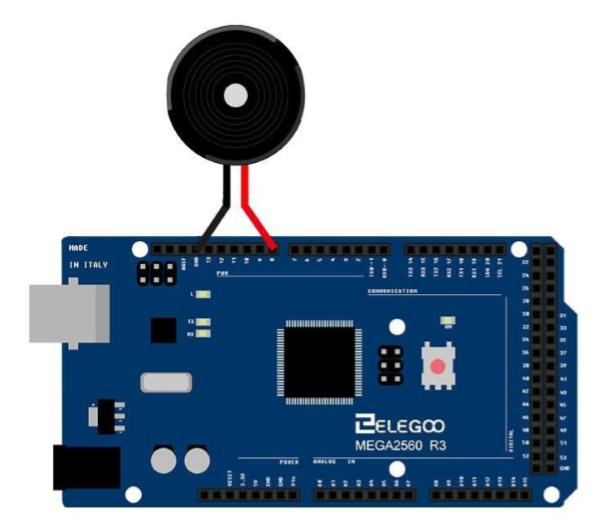
\includegraphics[width=1.0\textwidth]{./imagenes/3}
	\end{figure}
	
	%-----------------------------------------------------------------------
	%							BIBLIOGRAFIA
	%-----------------------------------------------------------------------
	% Referencia a bibliografia			En \cite{Baz}
	% Referencia a figura				La figura (\ref{fig:1})
	% Espacio entre lineas				\vspace{0.06in}
	% Figura con comentario al pie
	%\begin{figure}[htb]
	%	\centering
	%	
\includegraphics[width=0.4\textwidth]{./imagenes/1}
	%	\caption{Universidad de Granada.} \label{fig:1}
	%\end{figure}
	%\begin{thebibliography}{99}
	%	\bibitem{Baz} 
	%	\textsc{Bazaraa, M.S., J.J. Jarvis}
	%	\textit{Programacuib}.
	%	\newline
	%	\url{https://www.google.es}	
	%\end{thebibliography}

	


\end{document}